


\documentclass[a4paper,11pt]{article}
 \pdfoutput=1 % if your are submitting a pdflatex (i.e. if you have
             % images in pdf, png or jpg format)
\usepackage{jinstpub} 


% for details on the use of the package, please
                     % see the JINST-author-manual



\title{The Readout system of the CBM Projectile Spectator Detector at FAIR}


\author[a,c,1]{D. Finogeev,\note{Corresponding author.}}
\author[a,b]{F. Guber,}
\author[a]{N. Karpushkin,}
\author[a,b]{A. Makhnev,}
\author[a,c]{S. Morozov,}
\author[a]{D. Serebryakov,}

\affiliation[a]{Institute for Nuclear Research RAS, Moscow, Russia,}
\affiliation[b]{Moscow Institute of Physics and Technology, Dolgoprudny, Moscow Region, Russia}
\affiliation[c]{National Research Nuclear University MEPhI, Moscow, Russia}
\affiliation[d]{ Joint Institute for Nuclear Research, Dubna, Russia}


% e-mail addresses: only for the corresponding author
\emailAdd{dmitry.finogeev@cern.ch}




\abstract{The Projectile Spectator Detector (PSD) is a sampling lead/scintillator forward hadron calorimeter with transverse and longitudinal segmentation and with MPPCs photodetectors light readout. The PSD will be used at the Compressed Baryonic Matter (CBM) experiment at FAIR to measure the nucleus-nucleus collision centrality and orientation of the reaction plane. The CBM experiment will use a free-streaming data acquisition system (DAQ), which requires a coordinated time stamping of data in all sub-systems. To test prototypes of the CBM sub-detectors, FEE and readout electronics at high heavy ion beam rates the "mini CBM" (mCBM) installation has been assembled at SIS18 accelerator in GSI, Darmstadt, Germany in the framework of the FAIRPhase-0 program. A single PSD module (mPSD) has been integrated into the mCBM experiment. Details of the mPSD readout electronics and the first results of the data acquisition, processing and transmission within the common, synchronized mCBM data transport system taken during the first beam tests are shown. }



\keywords{Hadron calorimeters, trigger-less readout, GBT readout}

\collaboration[c]{on behalf of CBM collaboration}



\begin{document}
\maketitle
\flushbottom

\section{The CBM experiment at FAIR}
\label{sec:intro}
The future Compressed Baryonic Matter (CBM) experiment at the Facility for Antiproton and Ion Research (FAIR) is aimed to explore the Quantum Chromodynamics (QCD) phase diagram in the region of high baryon densities \cite{1}. The CBM will operate in the beam energy range of 2 - 11 AGeV and heavy ion interaction rates up to 10 MHz. The CBM experiment will use a free-streaming data acquisition system (DAQ), which requires a coordinated time stamping of data in all sub-systems. This coordination includes time-stamping against related clocks (common base), a synchronization procedure (deterministic time offsets) and the delivery of data containers of identical size during the data taking.


\section{The mCBM@SIS18 experiment}
The mCBM@SIS18 is a full-system test for CBM at the GSI/FAIR, comprised of detector modules from all CBM detector subsystems (MVD, STS, RICH, MUCH, TRD, TOF, ECAL, PSD). All subdetectors, excluding the mPSD, are positioned downstream of a target at an angle of 25◦ with respect to the beam axis. One module of PSD (mPSD) is placed under the beam axis at angle 5 degree relative the beam axis. The schematic view of mCBM is shown in the figure~\ref{fig:1}.

The mCBM setup will allow to test the most important aspects of CBM development \cite{2}:
\begin{itemize}
	\item Operation of the detector prototypes in a high-rate nucleus-nucleus collision environment
	\item Free-streaming data acquisition system including the data transport to a high-performance computer farm located in the "Green IT Cube"
	\item Online track and event reconstruction as well as event selection algorithms
	\item Offline data analysis
	\item Detector control system
\end{itemize}

\begin{figure}[htbp]
	\centering 
	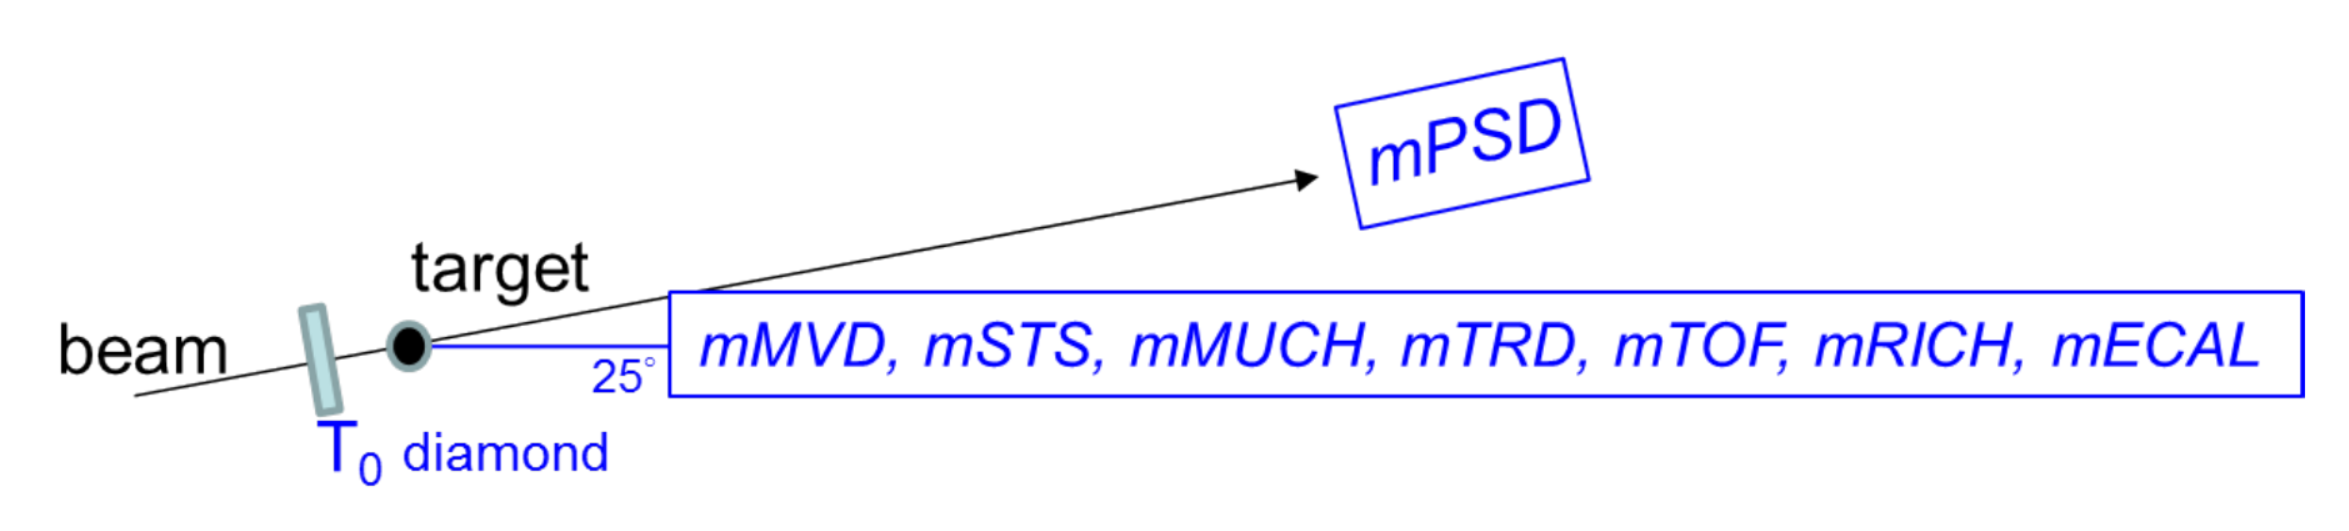
\includegraphics[width=.8\textwidth]{mCBM_sketch.png}
	\caption{\label{fig:1} Concept sketch of the proposed mCBM test-setup}
\end{figure}

To make possible the CBM@FAIR data collection with nucleus-nucleus collision rate up to 10MHz leading to a data rate up to 1TB per second, the ultra-fast and radiation tolerant GBTx ASIC data aggregation unit developed at CERN will be used. Afterwards, the data streams are handled by Data Processing Boards (DPB) containing powerful FPGAs and are forwarded via FLES Input Selector (FLES) which performs on-line event selection. In 2020-2021 DPB and FLIB will be replaced by a prototype of the Common Readout Interface (CRI) as it is foreseen in CBM experiment.


\section{The Projectile spectator detector at the CBM}
The PSD (the Projectile Spectator Detector) is the forward hadron compensating lead/scintillator calorimeter, which will be used in the CBM experiment to measure the centrality and the reaction plane orientation in heavy-ion collisions \cite{3}. The PSD has transverse and longitudinal segmentation with light readout performed via the micropixel photodetectors. 
The PSD will be assembled from already constructed 46 individual modules and has the beam hole in the center, as presented in figure ~\ref{fig:2}. Each module consists out of 60 lead/scintillator samples with 4 mm thick scintillator plate and 16 mm thick lead plate. Total length of module is about 5.6 nuclear interaction lengths. The transverse size of the module is 200x200 mm\textsuperscript{2} and the weight about 500 kg. Light from each scintillator plate is collected by the WLS-fiber glued in the circle groove in the scintillator plate and stretched in the 2 mm air gap at one the lateral sides of the module. Six consecutive scintillator tiles form a section and are collected together on separate optical connector at the end of the module. One Hamamatsu MPPC S12572-010P with active area 3×3mm\textsuperscript{2} is used as photodetector for each section of module. In addition, one optical fiber for the calibration system is glued into the same optical connector in addition to these 6 WLS-fibers. Other ends of 10 such fibers are collected together on separate optical connector to be illuminated by the light emitting diode (LED). 


\begin{figure}[htbp]
\centering % \begin{center}/\end{center} takes some additional vertical space
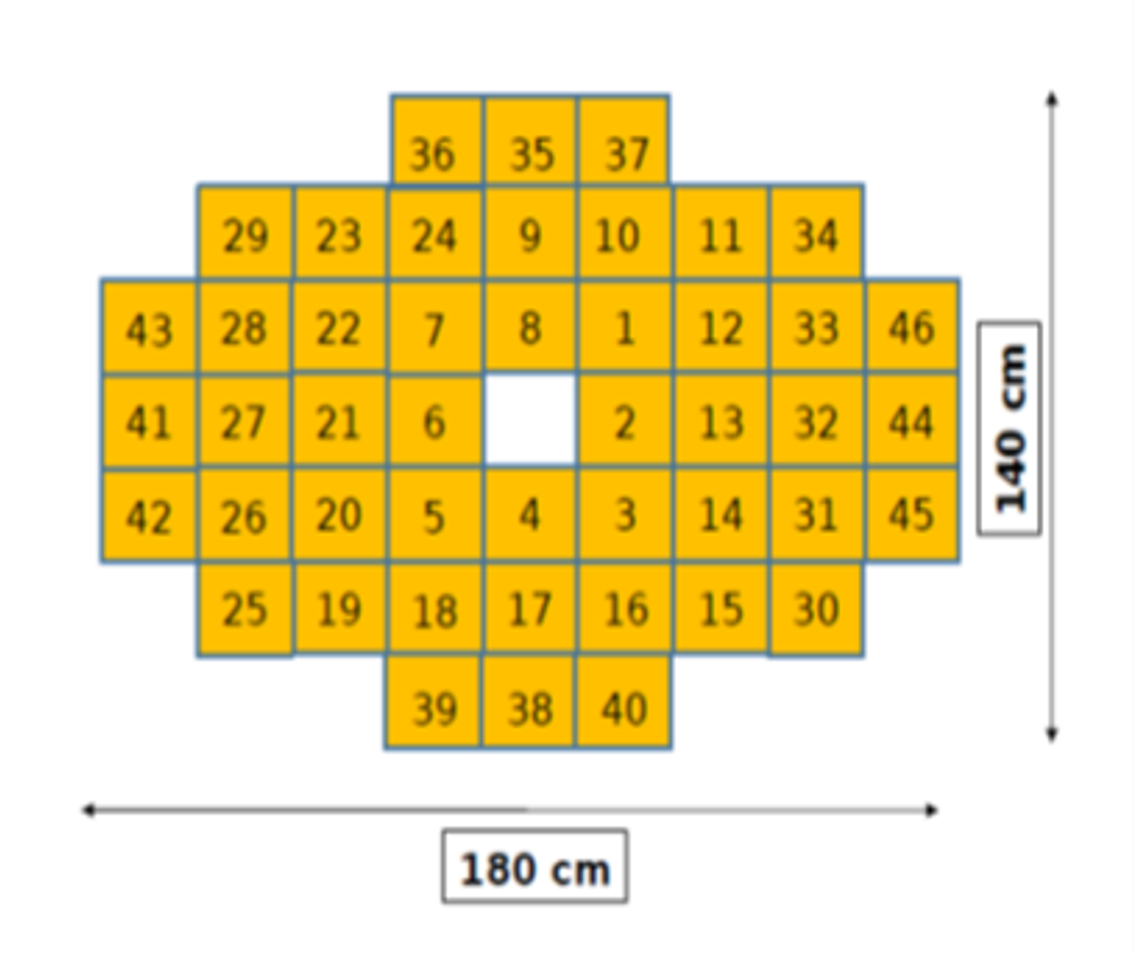
\includegraphics[width=.3\textwidth]{PSD_CBM_sketch.png}
\qquad
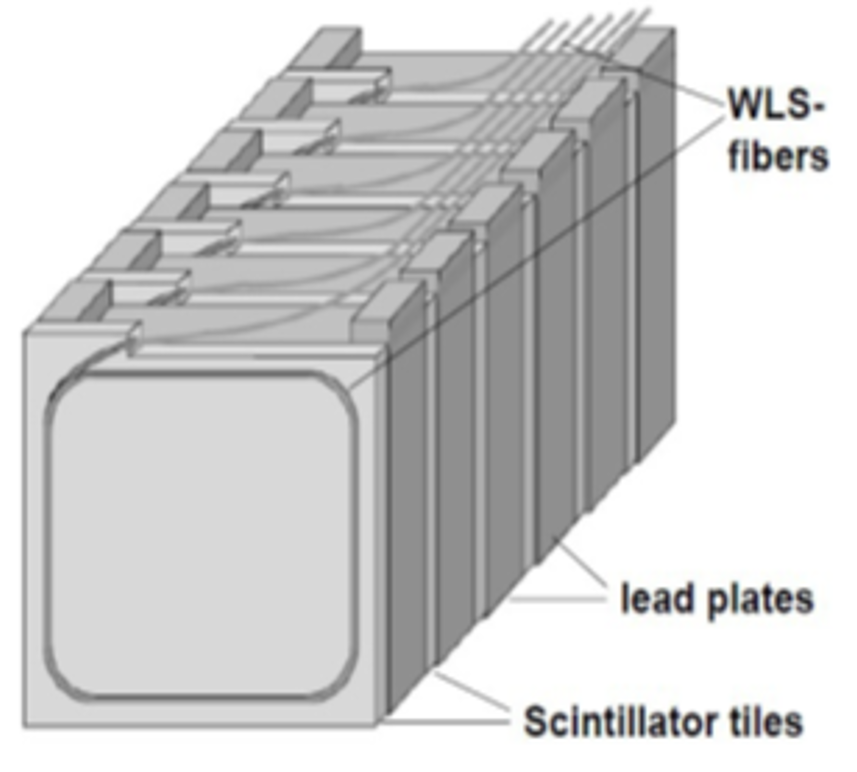
\includegraphics[width=.25\textwidth]{PSD_module_sketch.png}
\qquad
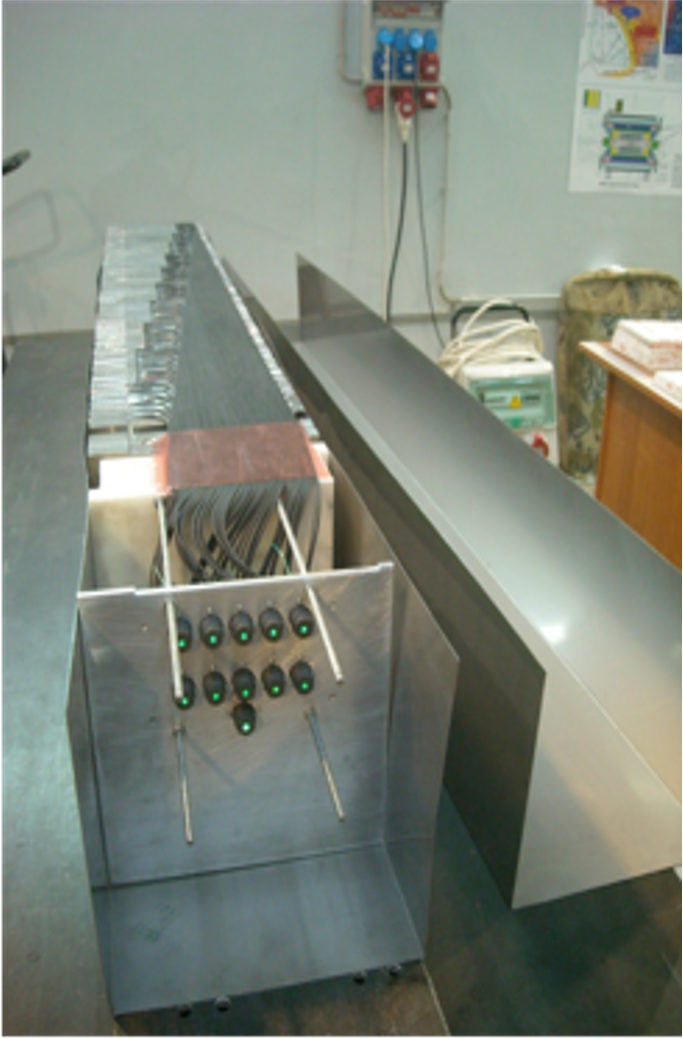
\includegraphics[width=.15\textwidth]{PSD_module_photo.png}
\caption{\label{fig:2} Schematic view of the CBM PSD, left. Schematic view of the PSD module structure, center. Photo of assembled PSD module, right}
\end{figure}

Each photodetector is supplied with a common reference voltage of about 70 volts, as well as individual automatic correction of the reference voltage depending on the external temperature. The temperature sensor, as well as the LED for the possibility of photoelectronic calibration of photodiodes, are placed on the FEE panel. The monitoring and data collection from all FEEs are carried out by means of the slow control system.
The monitoring system provides the MPPCs gain control during the data taking. Thus, each PSD module has ten longitudinal sections, which ensures the uniformity of light collection along the modules. Schematic view and photo of a PSD module without top cap are shown in figure~\ref{fig:2}, center and right.




\section{PSD readout concept}
Signal readout is performed with an ADC board represented in figure~\ref{fig:3} (left) and an Addon board represented in figure~\ref{fig:3} (right). Estimated accumulated neutron flux for 2 months of operation is $10^11$ for board with MPPC. To avoid radiation influence to electronics, FEE and ADC readout boards will be distanced from calorimeter to 25 - 40 m. Signals from MPPCs are collected by the ADC Addon board, which provides a single-ended interface based on single-ended to differential converters AD8138 ICs. Design allows for an adjustable input and output offset, utilizing the whole dynamic range of the converter. Besides providing a signal interface, Addon board includes an MPPC offset adjustment system, that consists out of 16 four-channel digital to analog converters (DACs) with unity-gain buffers. DACs provide a DC offset on the signal line, regulating voltage over the MPPC's terminals. Control of the DACs is accomplished through an STM32F103 microcontroller placed on the Addon board, which receives commands and adjustment data from the ADC board.

Signals are then digitized by the ADC board initially designed for the ECAL detector of PANDA experiment \cite{4} (see figure~\ref{fig:3}, left). The 64-channel board based on ADC LTM9011 with digitization rate up to 125Msps and 14-bit digitization resolution. The ADC board is mounted directly onto the Addon board (see figure~\ref{fig:3}, right), and the whole assembly is designed to fit standard 6U Eurocard cradles.
Digitized samples of 64 analog signals are sent to 2 Kintex 7 FPGAs  using 128 LVDS links. Each FPGA processes data from 32 channels. Signal
processing algorithm is based on the Prony-LS fitting procedure \cite{5}, which allows working with signals near the noise level, and is also used for the pile-up recognition. Such algorithm will be implemented in the FPGA firmware in the future.
To meet the requirements of experiment's DAQ, GBT FPGA transceiver was integrated into the firmware. GBT allows to transmit data, slow control and clock signals. Expected data rate is 1MHz per channel that gives a constrain of 100bit/hit for GBT data rate of 3.2 Gbit/s. 
LMK0460 jitter cleaner used for generation of ADC and MGTREF clocks. After a reset signal, 100MHz clock from on-board generator TD-100 is used as a master clock. After GBT RX synchronization is established, source is switched to external clock, sourced from GBT RX. The clock switching scheme allows to maintain common DAQ clock domain. Measuring hit time in trigger-less readout occurs relative to the time counting named "timeslice", which is synchronized for the whole experiment readout.

\begin{figure}[htbp]
	\centering
	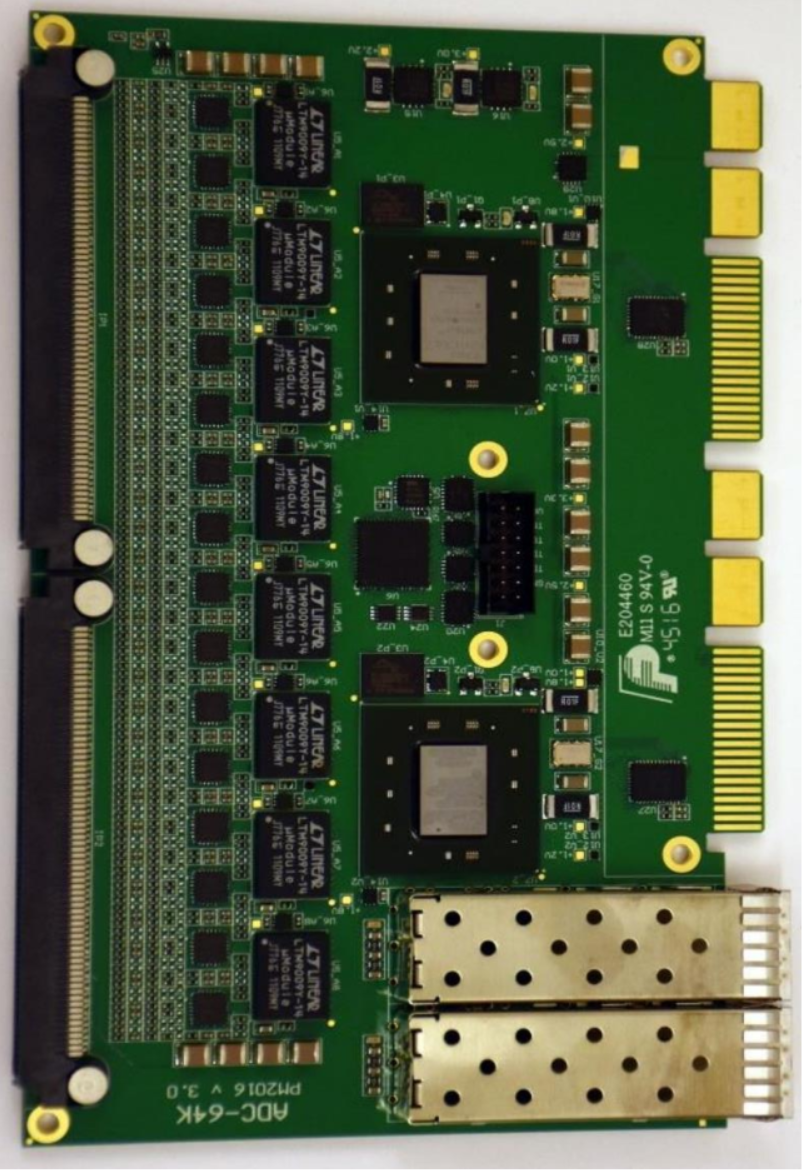
\includegraphics[width=.3\textwidth]{ADC_board.png}
	\quad
	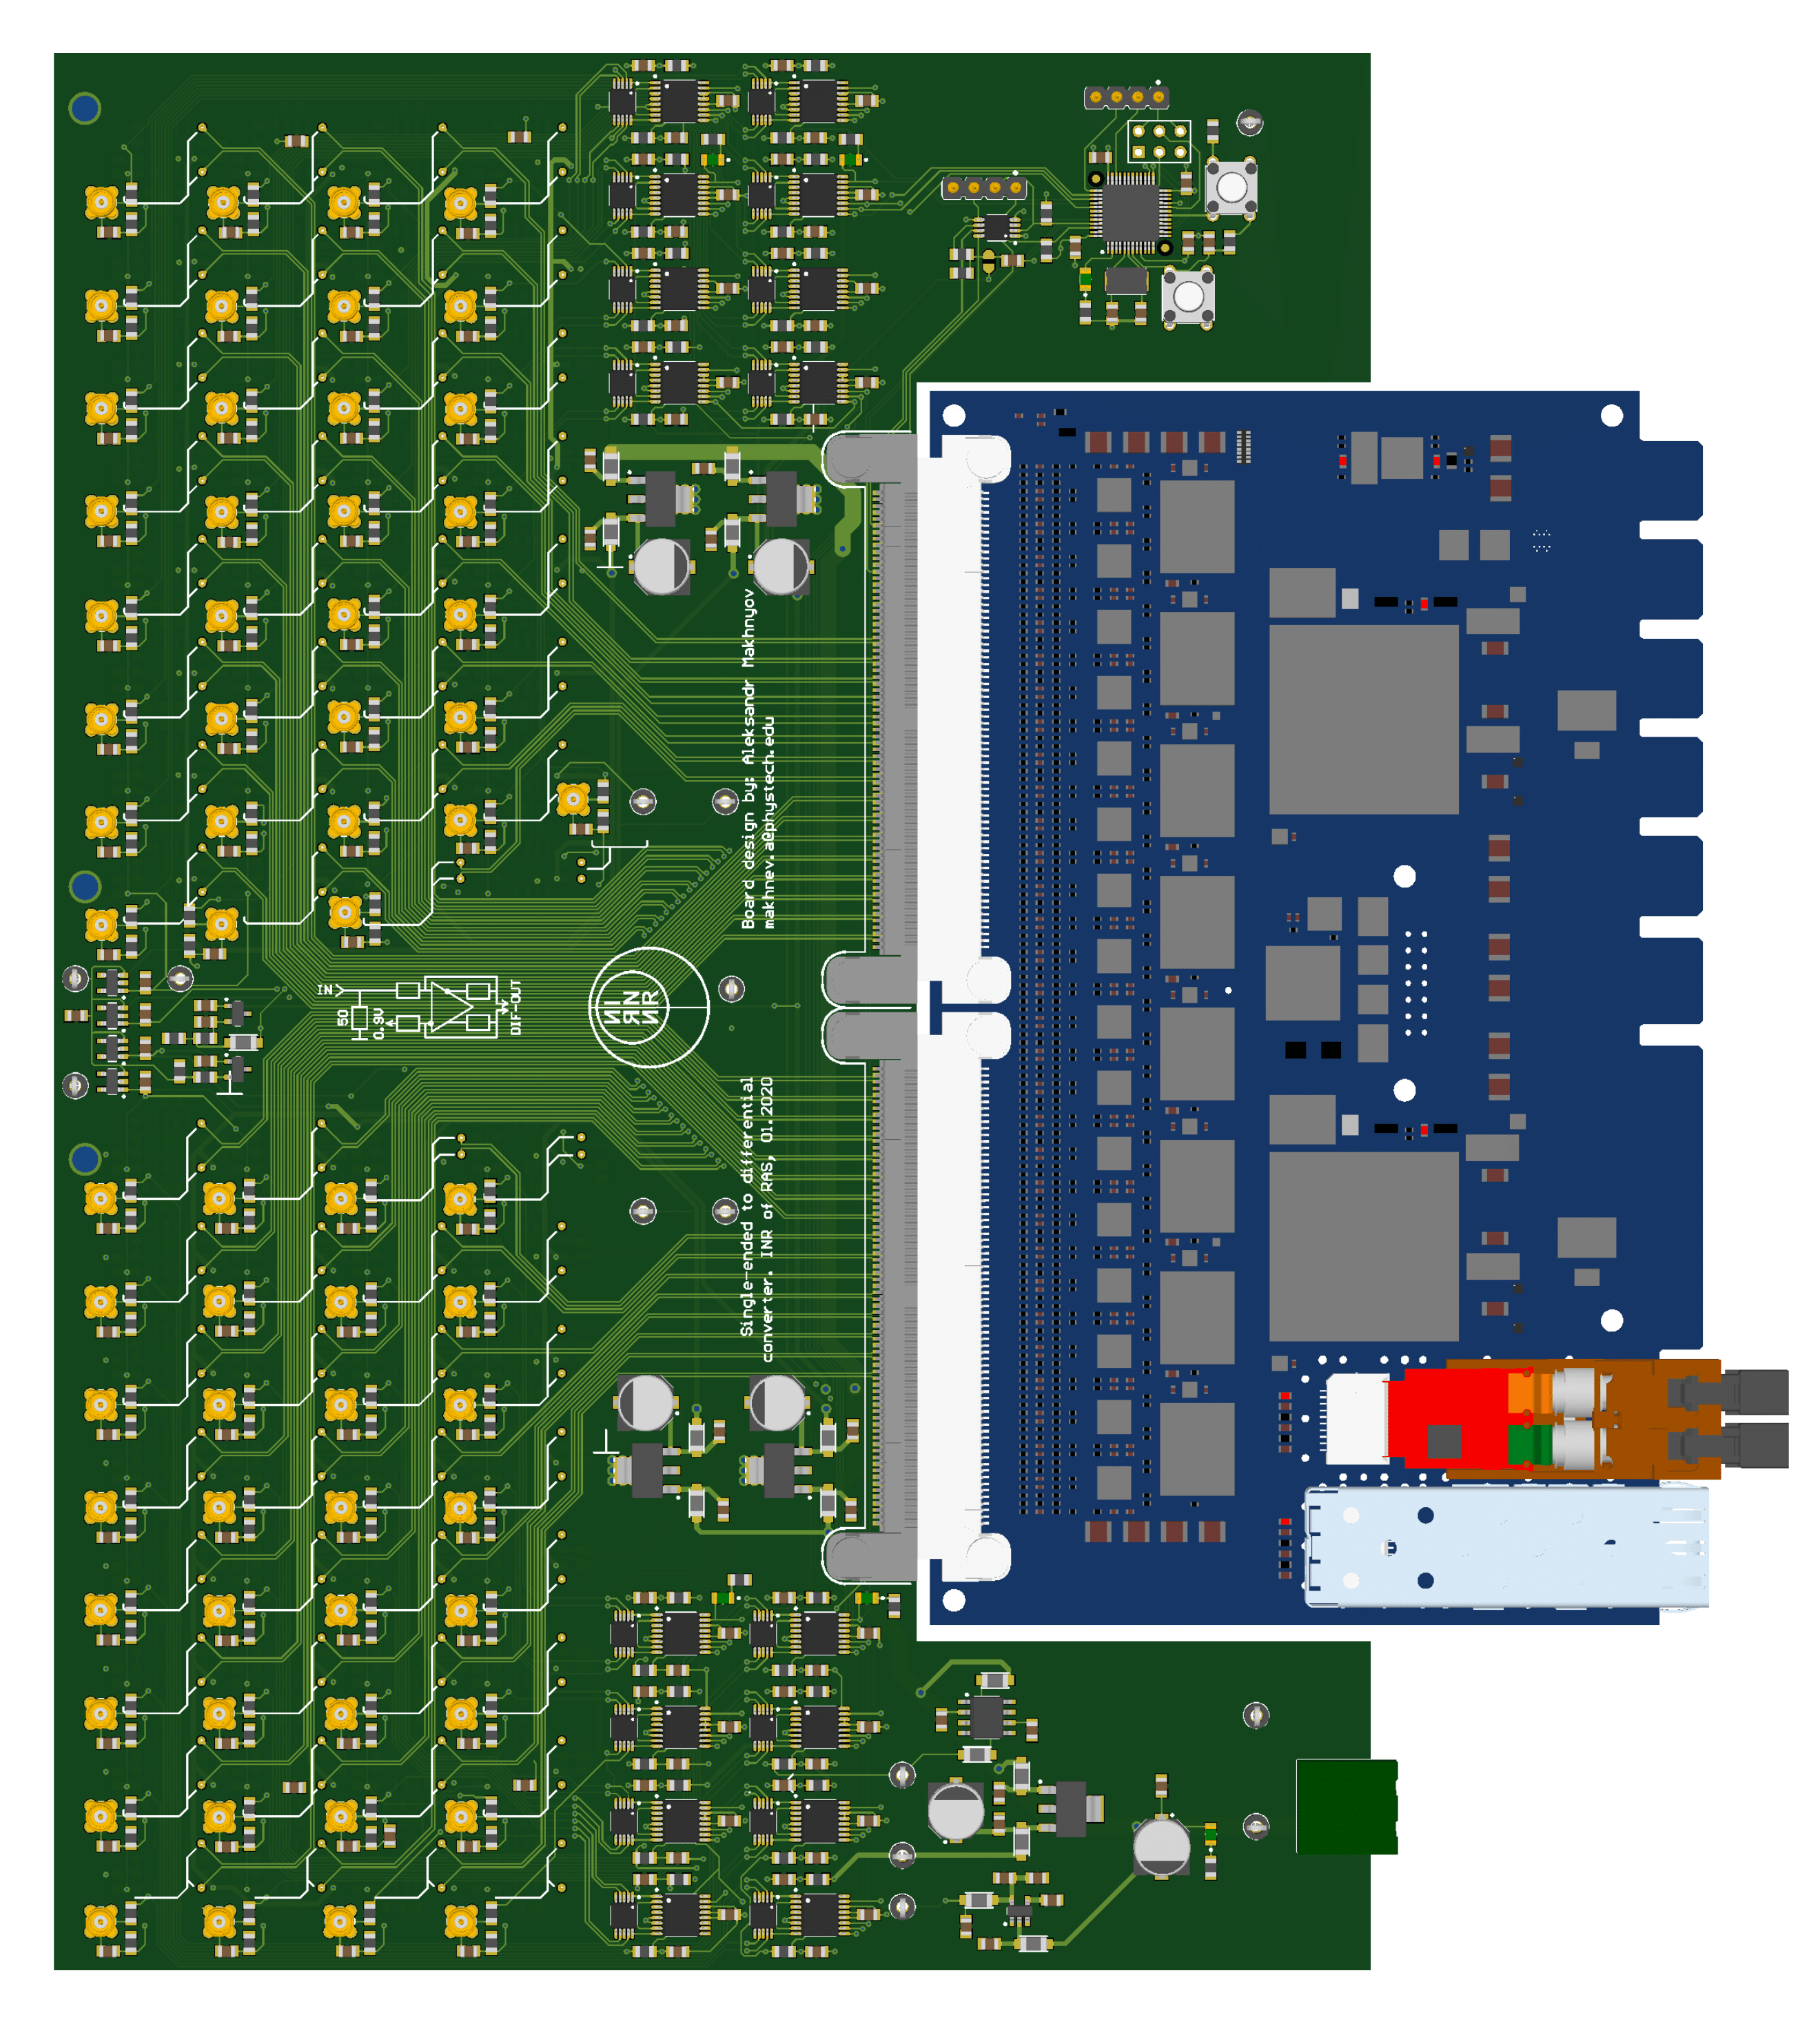
\includegraphics[width=.4\textwidth]{ADC_addon.png}
	\caption{\label{fig:3} 64-channel ADC board with 2 FPGA Kintex 7 (left); Addon board design with the ADC board mounted (right)}
\end{figure}

\section{ The first mPSD beam test results at mCBM}
At the end of 2019 and beginning of 2020 beam tests at mCBM@SIS18 were carried out with Au and Pb ions at 1.01 - 1.22 AGeV energy range. The main goal is to test detectors subsystems, DAQ and online data aggregation procedure. Test of the mPSD prototype as part of mCBM experiment allows to approve and verify the feasibility of the PSD readout concept. The prototype includes crucial parts of the readout such as Addon prototype board and ADC FPGA readout board. In this setup, Addon incorporated only the single-ended to differential converters and the necessary power systems. Photo of the assembled FEE setup is represented on figure~\ref{fig:4}.

\begin{figure}[htbp]
\centering % \begin{center}/\end{center} takes some additional vertical space
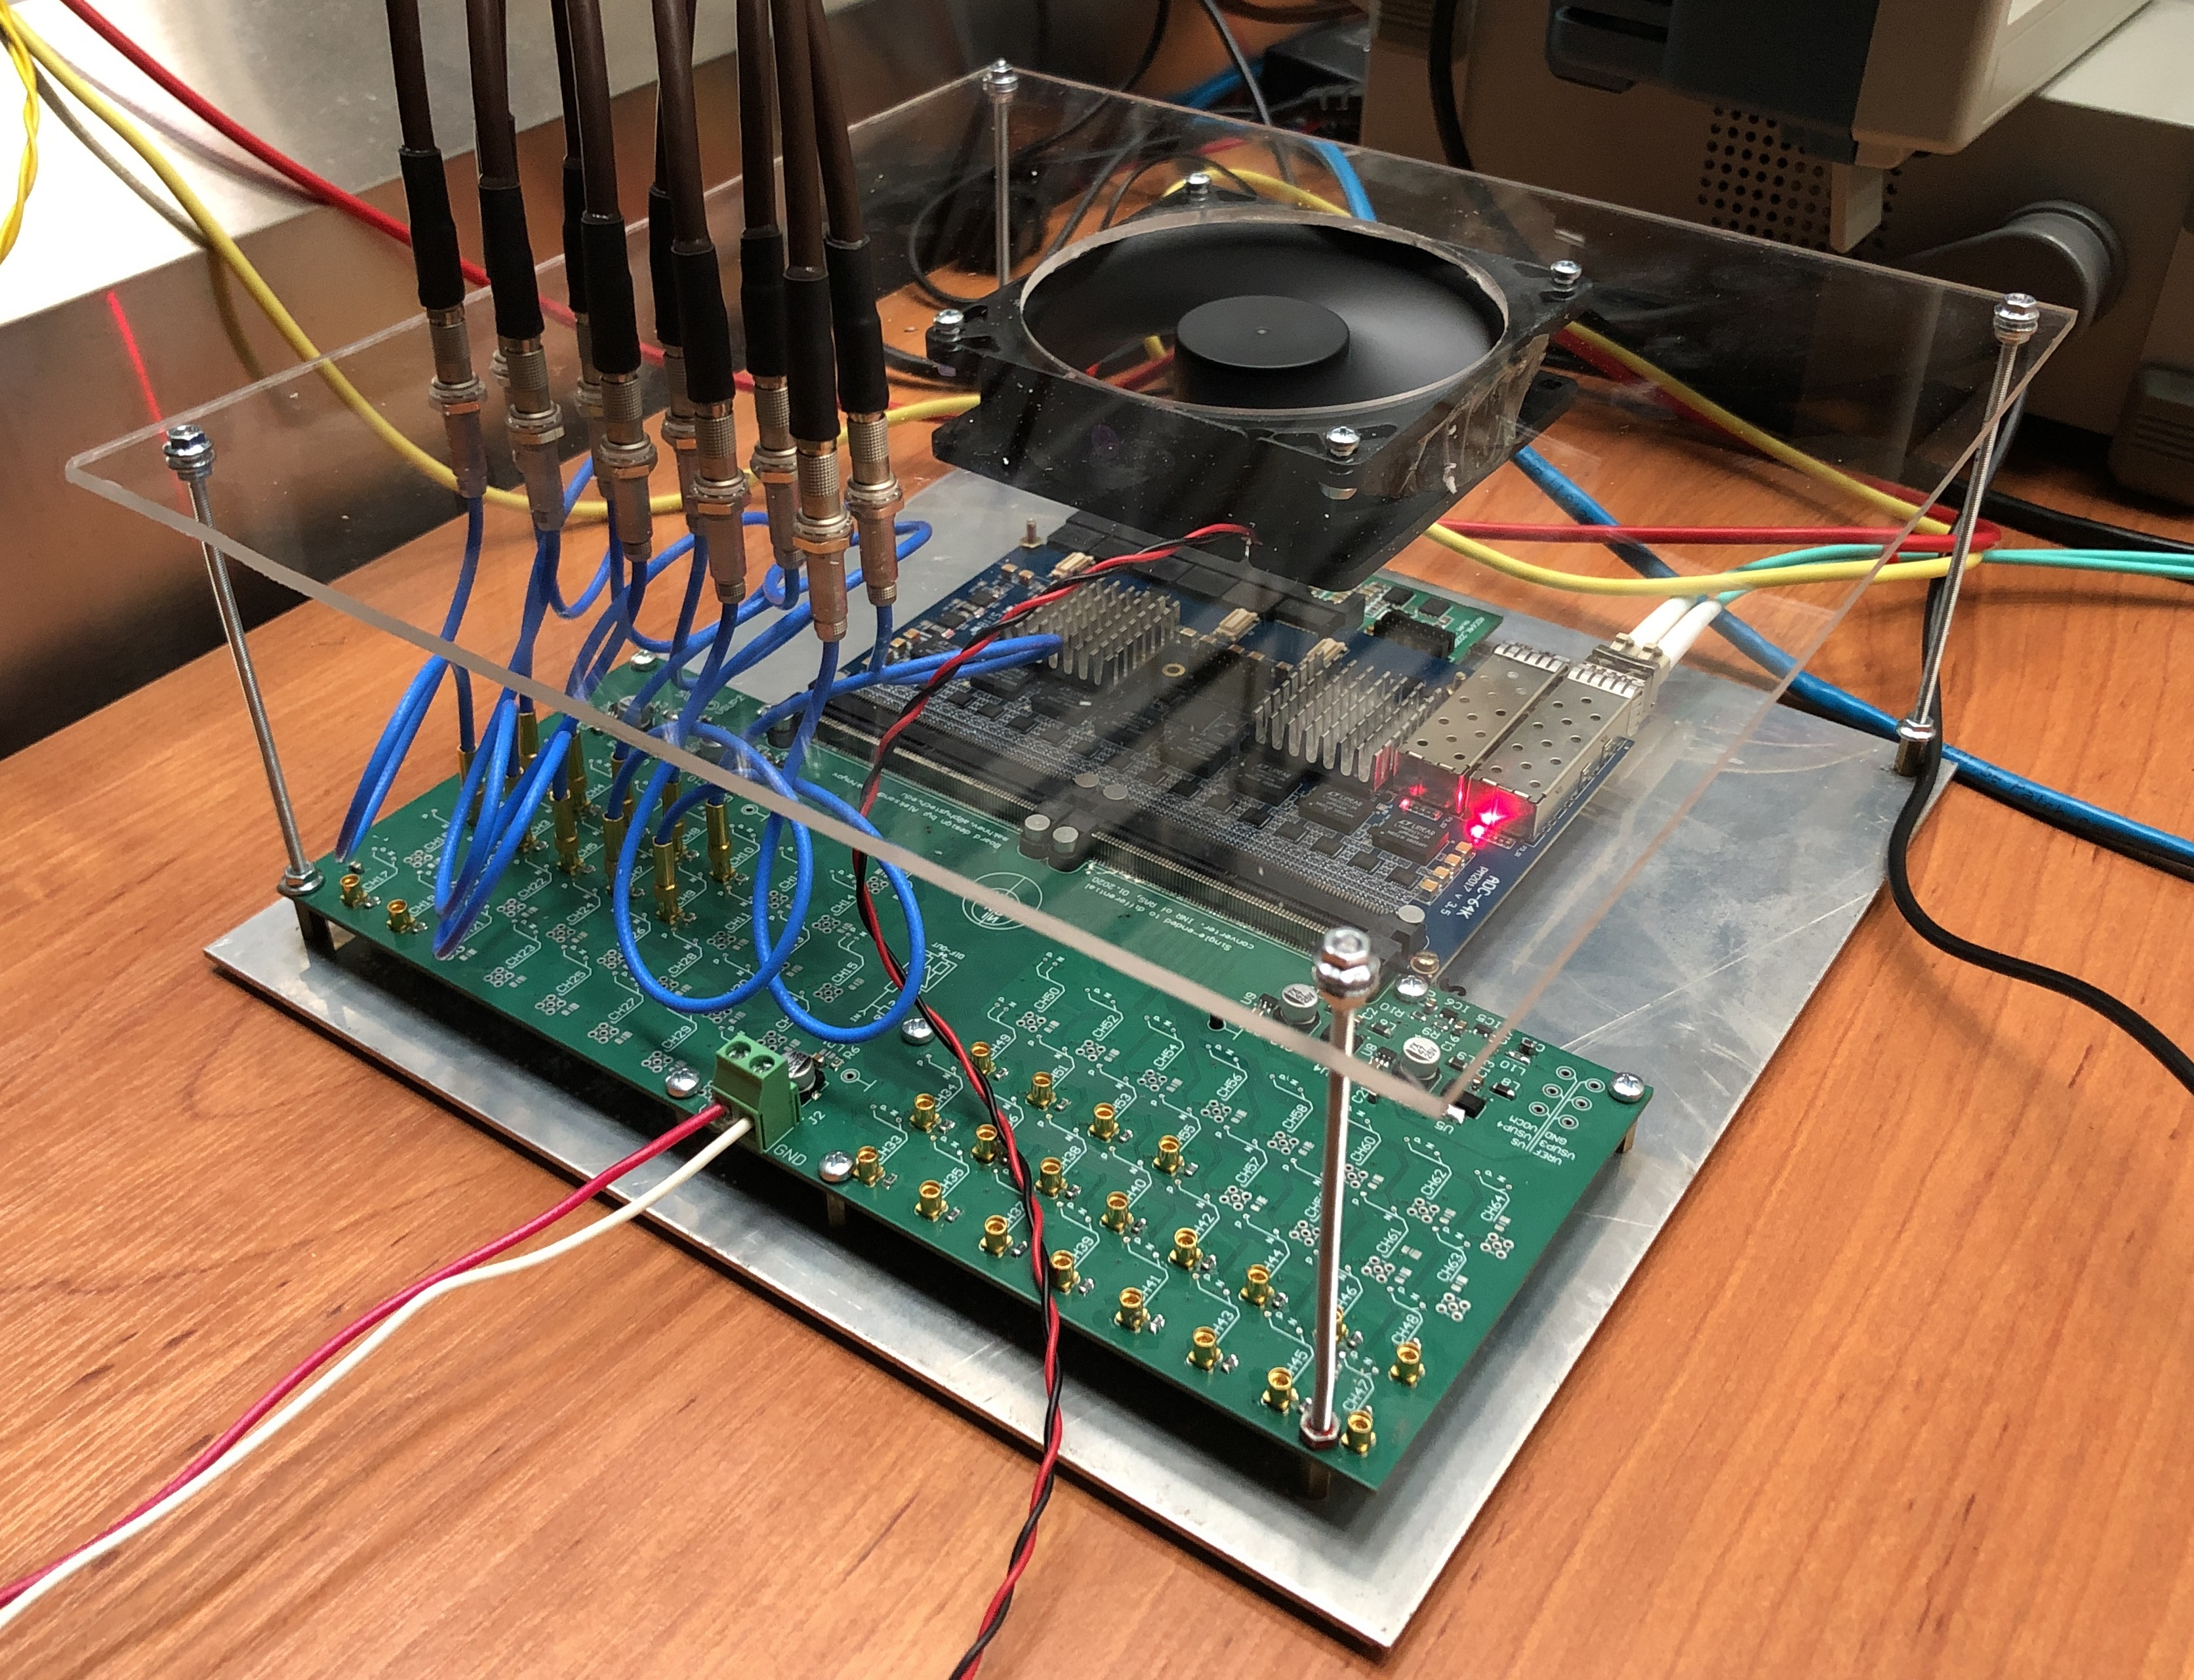
\includegraphics[width=.5\textwidth]{mPSD_FEE_photo.JPG}
\qquad
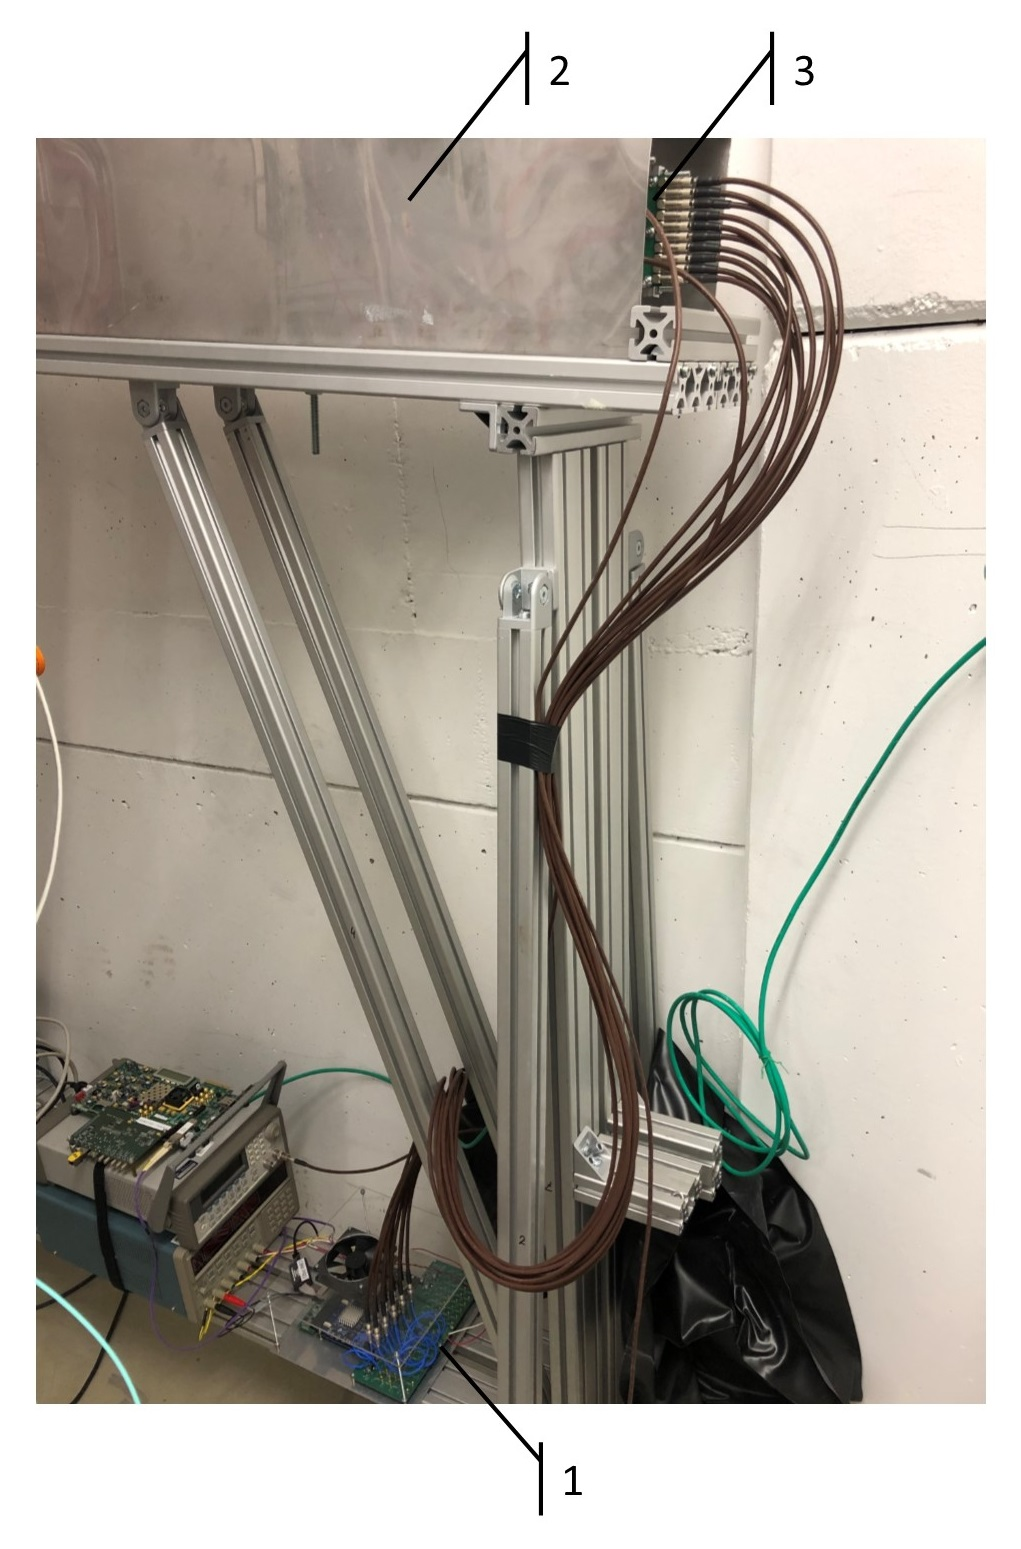
\includegraphics[width=.4\textwidth]{mPSD_module_photo.JPG}
\caption{\label{fig:4} Photo of the ADC board assembled with the Addon board prototype (left); photo of mPSD module connected to FEE}
\end{figure}

ADC FPGA board was connected to mCBM DAQ via GBT protocol used for data transport, clock distribution and configuration purposes. ADC was used in 80 Msps digitization mode, with an upgrade up to 120 Msps scheduled in 2020. Each channel is triggered independently by amplitude threshold crossing and extracts energy data from the waveform of the input signal measured in a fixed gate. ADC takes data in trigger-less readout mode according to CBM DAQ requirements. Also prototypes of all crucial software parts such data unpacker, event building and data monitor was developed and tested.

\subsection{PSD data monitoring}
Information of the mPSD detector is transmitted to the mCBM common data reading system using the DPB board with modified firmware. Currently, mPSD data packages are sets of 64-bit messages containing information about the time stamp of the signal, total number and indices of triggered channels, charges, zero levels and times of the signal's arrival, as well as the information about the signal's waveforms.
The completeness and integrity of the received data packets is monitored by the number of read GBT words. In addition, control of all transmitted information is also carried out online through a software module developed for data monitoring (see figure~\ref{fig:5}). The top two graphs serve here to track the indices of triggered channels. The indices correspond to the PSD sections from 0 to 8. An external source was connected to channel 9, which serves to check the synchronization between the mCBM detectors. The lower left graph shows the distribution of energy deposition in PSD sections. The major part of the energy is deposited in the two front sections of the calorimeter. The bottom right graph shows the evolution of the length of the microslices. This information is used to verify data integrity.

\begin{figure}[htbp]
\centering % \begin{center}/\end{center} takes some additional vertical space
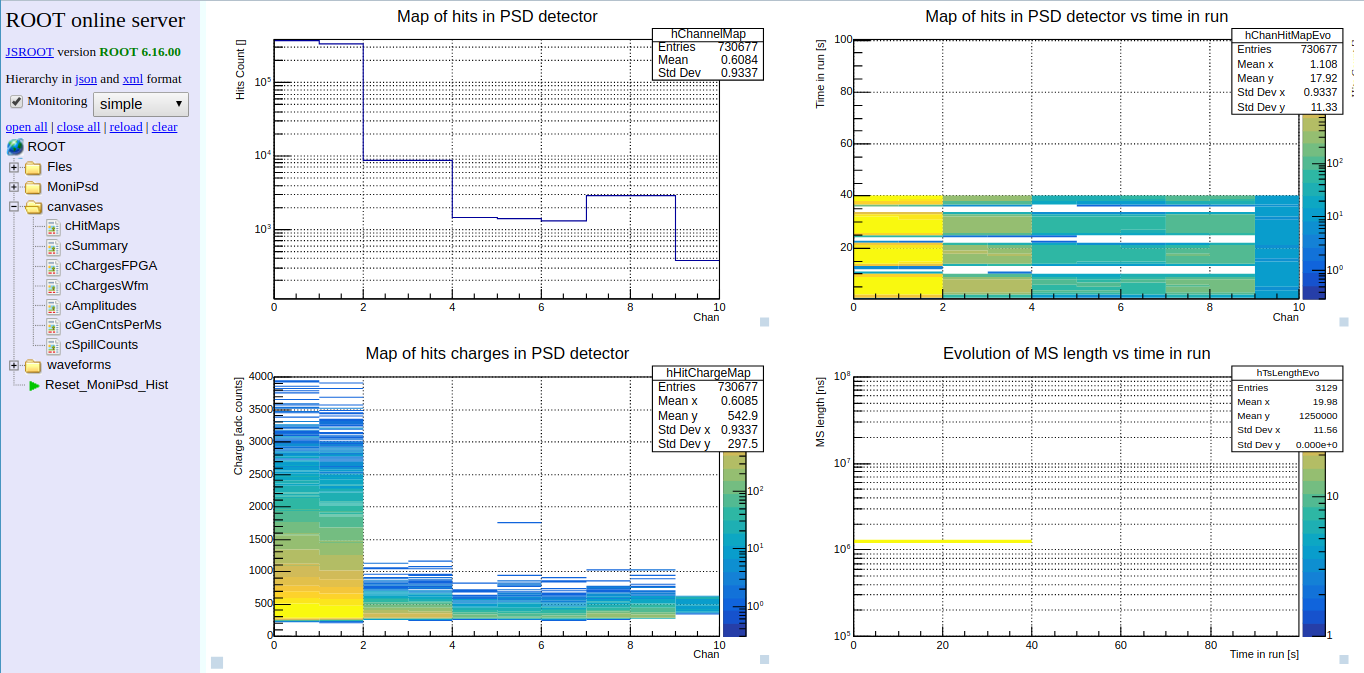
\includegraphics[width=\textwidth]{run582.png}
\caption{\label{fig:5} Data monitoring software module}
\end{figure}


\subsection{Preliminary mPSD test results}
One of the prime aims of mCBM is to test and validate the data processing concept and the reconstruction software which are being developed for the full CBM experiment. mCBM thus will be a demonstrator for the computing concept of CBM, including the reconstruction of events and selection of data in real-time and the full offline data analysis. It is thus planned to use already existing software components as far as possible for both online and offline computing in mCBM.
The challenge of the trigger-less readout is time synchronization and event building procedure. It is necessary to construct events from signals based on their time stamps while data processing.
During the data acquisition, information from all the detectors of the mCBM experiment is recorded in a common binary file. To check the synchronization of the data from the detectors, the time correlation graphs are constructed (see figure~\ref{fig:6}). An explicit peak in the distribution of the difference in the response time of the detectors T0 and PSD (time offset), located at about 200 ns, indicates the correlation of the data and serves to select beam events.
In the same way, the timestamps of signals from all subsystems are used to attribute these signals to a specific event. To ensure the possibility of this approach, time synchronization between the subsystems is used taking into account the time offsets that are inevitably introduced during the signal acquisition process. In the current approach, we assume the signals to form a single event, if their time stamps are located in a single time window of 200ns. In addition to introducing a fixed time window for event selection, conditions on the minimum number of signals from subsystems that are located in the considered time window can be applied. Such a straightforward approach is justified at the debugging stage and will be improved in the future.

\begin{figure}[htbp]
\centering % \begin{center}/\end{center} takes some additional vertical space
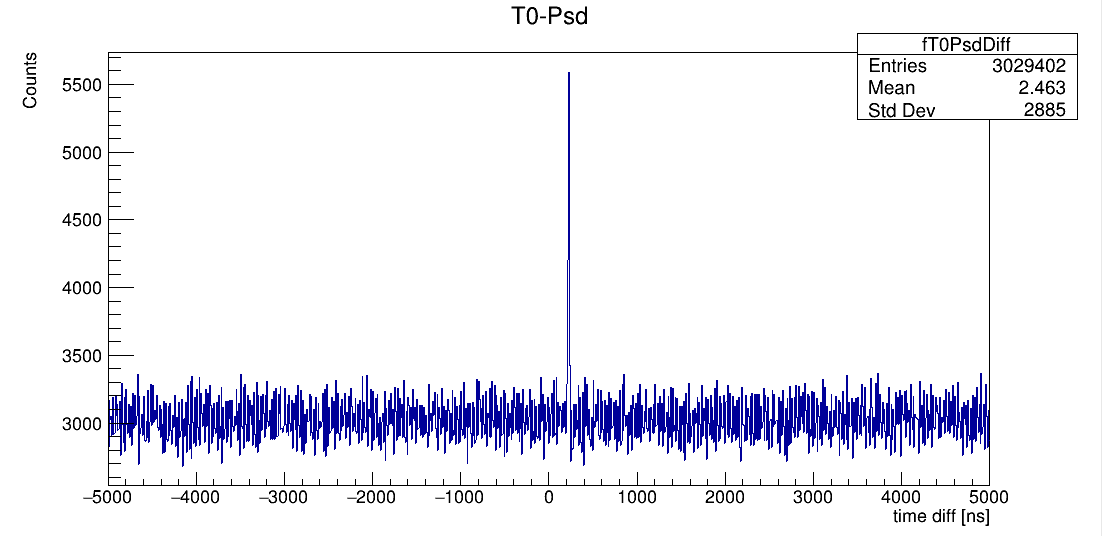
\includegraphics[width=\textwidth]{run582T0Psd.png}

\caption{\label{fig:6} T0-Psd time correlation}
\end{figure}

The distribution of mPSD energy deposition in events constructed is shown in figure~\ref{fig:7} (left). The presence of two peaks here is explained by the discrete number of triggered sections in the event. The right side of figure~\ref{fig:7} shows the energy profile in the mPSD sections.

\begin{figure}[htbp]
\centering % \begin{center}/\end{center} takes some additional vertical space
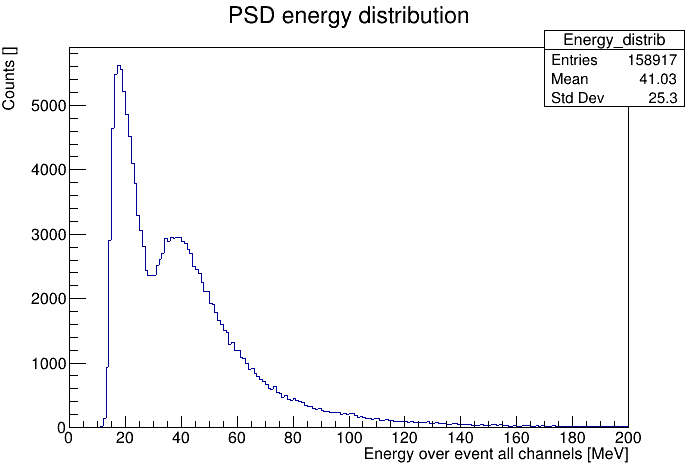
\includegraphics[width=.45\textwidth]{PsdEdepInEvent_calibrd.png}
\qquad
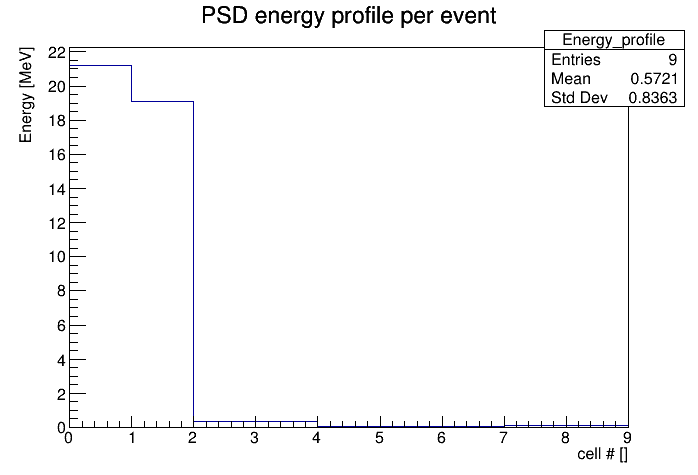
\includegraphics[width=.45\textwidth]{PsdEprofileInEvent_calibrd.png}
\caption{\label{fig:7} mPSD energy deposition (left); mPSD energy profile (right)}
\end{figure}

\section{Conclusions}
The prototype of mPSD@CBM readout system was implemented and tested n first high rate heavy ion interactions. mPSD beam tests included all conceptual hardware, firmware and software parts which will be used for final PSD@CBM setup developement. Signal transmission chain, ADC data processing on 80 Msps rate and GBT protocol functionality with clock switching procedure were tested. Preliminary results of the analysis of data collected on the test beams of the mCBM experiment in the trigger-less mode were presented. The approach to tracking the integrity and quality of the data being collected is described, as well as the principle of the formation of events by the signal's time stamps is shown.
Feasibility of the readout concept was proved and development of the full PSD readout system has been started.

\acknowledgments
We thank C. Sturm, D. Emschermann and P-A. Loizeau for help while mCBM test beam data taking.

\begin{thebibliography}{99}


\bibitem{1}
CBM Collaboration, T. Ablyazimov et al., \emph{Challenges in QCD matter physics -The scientific programme of the Compressed Baryonic Matter experiment at FAIR} Eur.Phys.J. A53 (2017) no.3, 60 


\bibitem{2}
C.Sturm et al., mCBM@SIS18, \emph{A CBM full system test-setup for high-rate nucleus-nucleus collisions at GSI / FAIR} http://www.fair-center.eu/fileadmin/fair/experiments/CBM/documents/mcbm-proposal2GPAC-WebVersion0619-SVN7729.pdf

\bibitem{3}
Guber F, et al., \emph{Technical Design Report for the CBM Projectile Spectator} https://repository.gsi.de/search?p=id:\%22GSI-2015-02020\%22

\bibitem{4}
Serneguet Sorli, Á. (2015). \emph{A multichannel digitizer for the PANDA experiment.} http://hdl.handle.net/10251/56722.

\bibitem{5}
\emph{Application of the Prony least squares method for fitting signal waveforms measured by sampling ADC}
October 2019AIP Conference Proceedings 2163(1):030006
DOI: 10.1063/1.5130092
Conference: PROCEEDINGS OF THE 23RD INTERNATIONAL SCIENTIFIC CONFERENCE OF YOUNG SCIENTISTS AND SPECIALISTS (AYSS-2019)



\end{thebibliography}
\end{document}

